\documentclass[main.tex]{subfiles}
\begin{document}
    \chapter{Lateral}
    \label{ch:lateral}
    
    Preliminary investigations of the lateral control subsystem included analysis of a double-sided linear induction motor (DSLIM) to provide both propulsion and lateral stability. For Goose III, a DSLIM was ultimately ruled out as the functional velocity range of most linear induction motors is much smaller than that of the pod, meaning that the lateral stabilization force provided by the DSLIM would become ineffective after a certain velocity.\\
    Lateral wheels were chosen for the final design as they allowed for a passive and lightweight lateral control system capable of supplying sufficient lateral forces to maintain stability.

    \section{Overall Design}
    \begin{figure}
    	\centering
        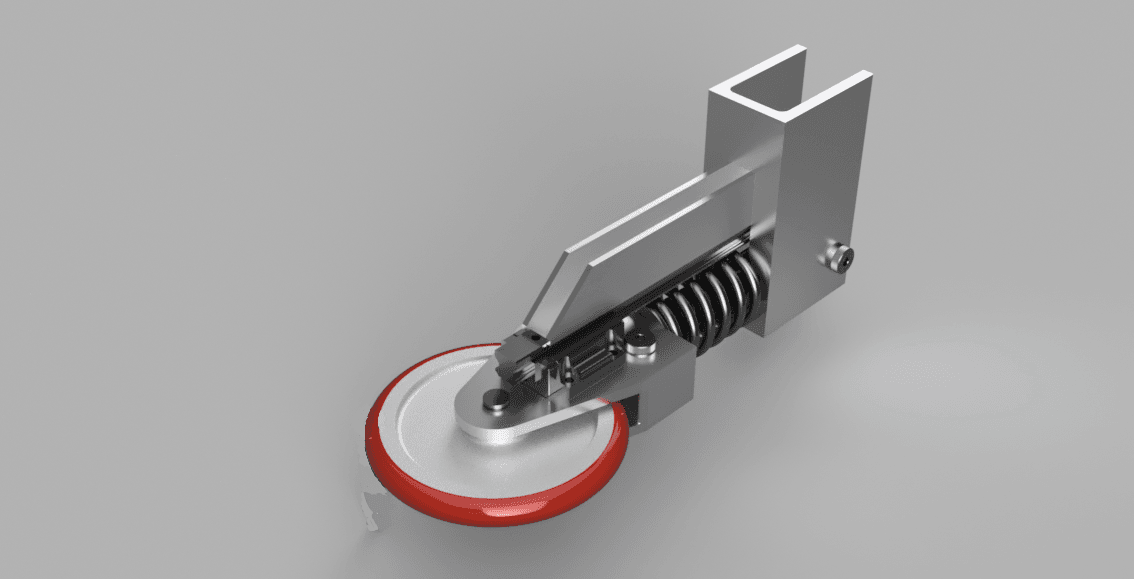
\includegraphics[width=\linewidth]{images/Lateral_Master}
        \label{fig:lateralMaster}
        \caption{The Lateral Subassembly.}
    \end{figure}
    The lateral control subassembly consists of an aluminum wheel being pressed against the web of the I-beam. The wheel and clevis assembly slides along a rail on a carriage. An adjustable damper is threaded into the clevis assembly on one end and fixed to the lateral mount on the other. The damper fits inside the spring and serves to dissipate the pod's lateral kinetic energy, while the spring serves to maintain the pod's equilibrium position.\\
    A full Bill of Materials can be found in \reftab{tab}.

    \section{Structural}
    \begin{figure}
    	\centering
        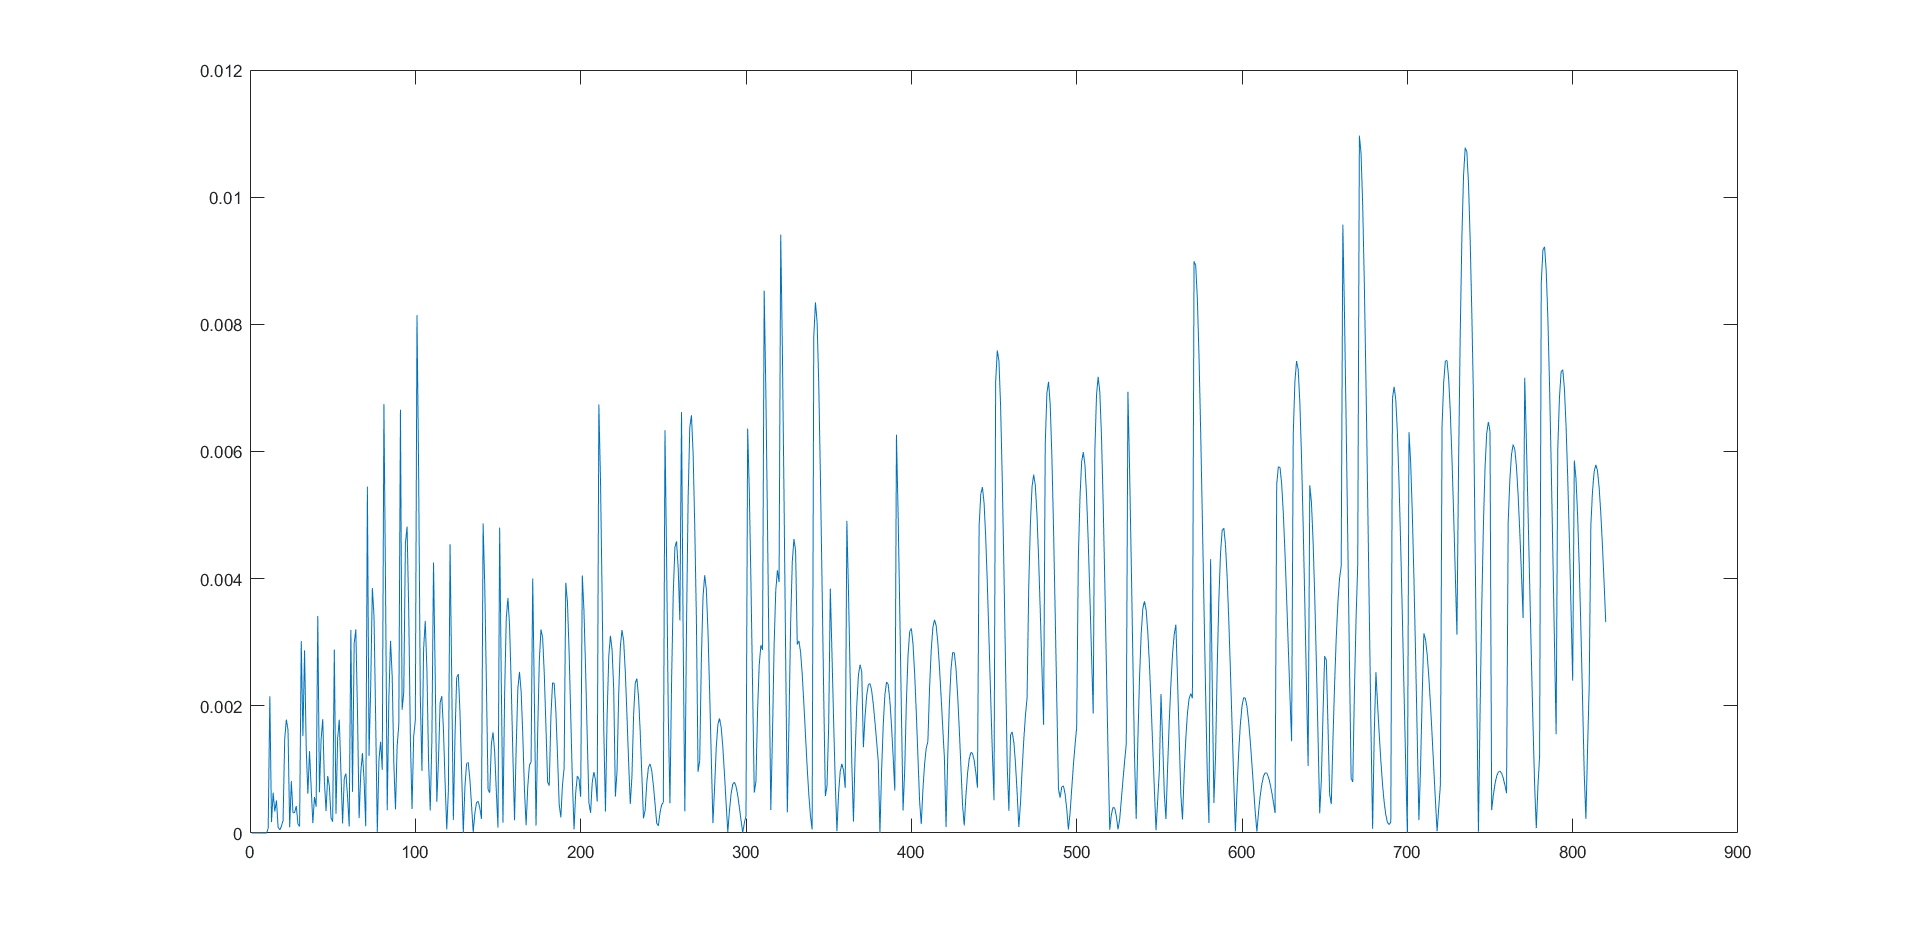
\includegraphics[width=\linewidth]{images/RandDistToRail}
        \label{fig:RandDistToRail}
        \caption{The plot of the distance to the rail in when the rails are arranged in a random order. We see that the lowest pod-rail distance is less than 12 millimetres; for reference, the brakes are nominally at 19mm when deployed.}
    \end{figure}
    MATLAB simulations were created to ensure the lateral control system would maintain a close distance to the rail so as to prevent any pod component from entering a no-go zone or colliding with the rail. For example, the Eddy Current Brakes (when deployed) have a nominal distance to the rail of 19mm. As such, the lateral control system must always maintain a distance smaller than 19mm, seen on Figure 5.2 on page 63.\\
    The MATLAB simulation is programmed with inputs of pod mass, pod acceleration, and spring and damper coefficients. The simulation models the pod's lateral position when subjected to rails which are offset by values two times those listed in the tube specification PDF. It is important to note that this simulation models the pods entire acceleration profile; it starts from rest and reaches the pod's top speed at the end of the graph, so the pod's lateral response behaviour appears to change along the graph. Because of this, the pod tends to return to equilibrium faster on the left portion of the graph. \\
    The rails can either be oscillating back and forth or randomly arranged. They can also be angled to a degree specified in the tube specifications PDF.\\
    \begin{figure}
        	\centering
        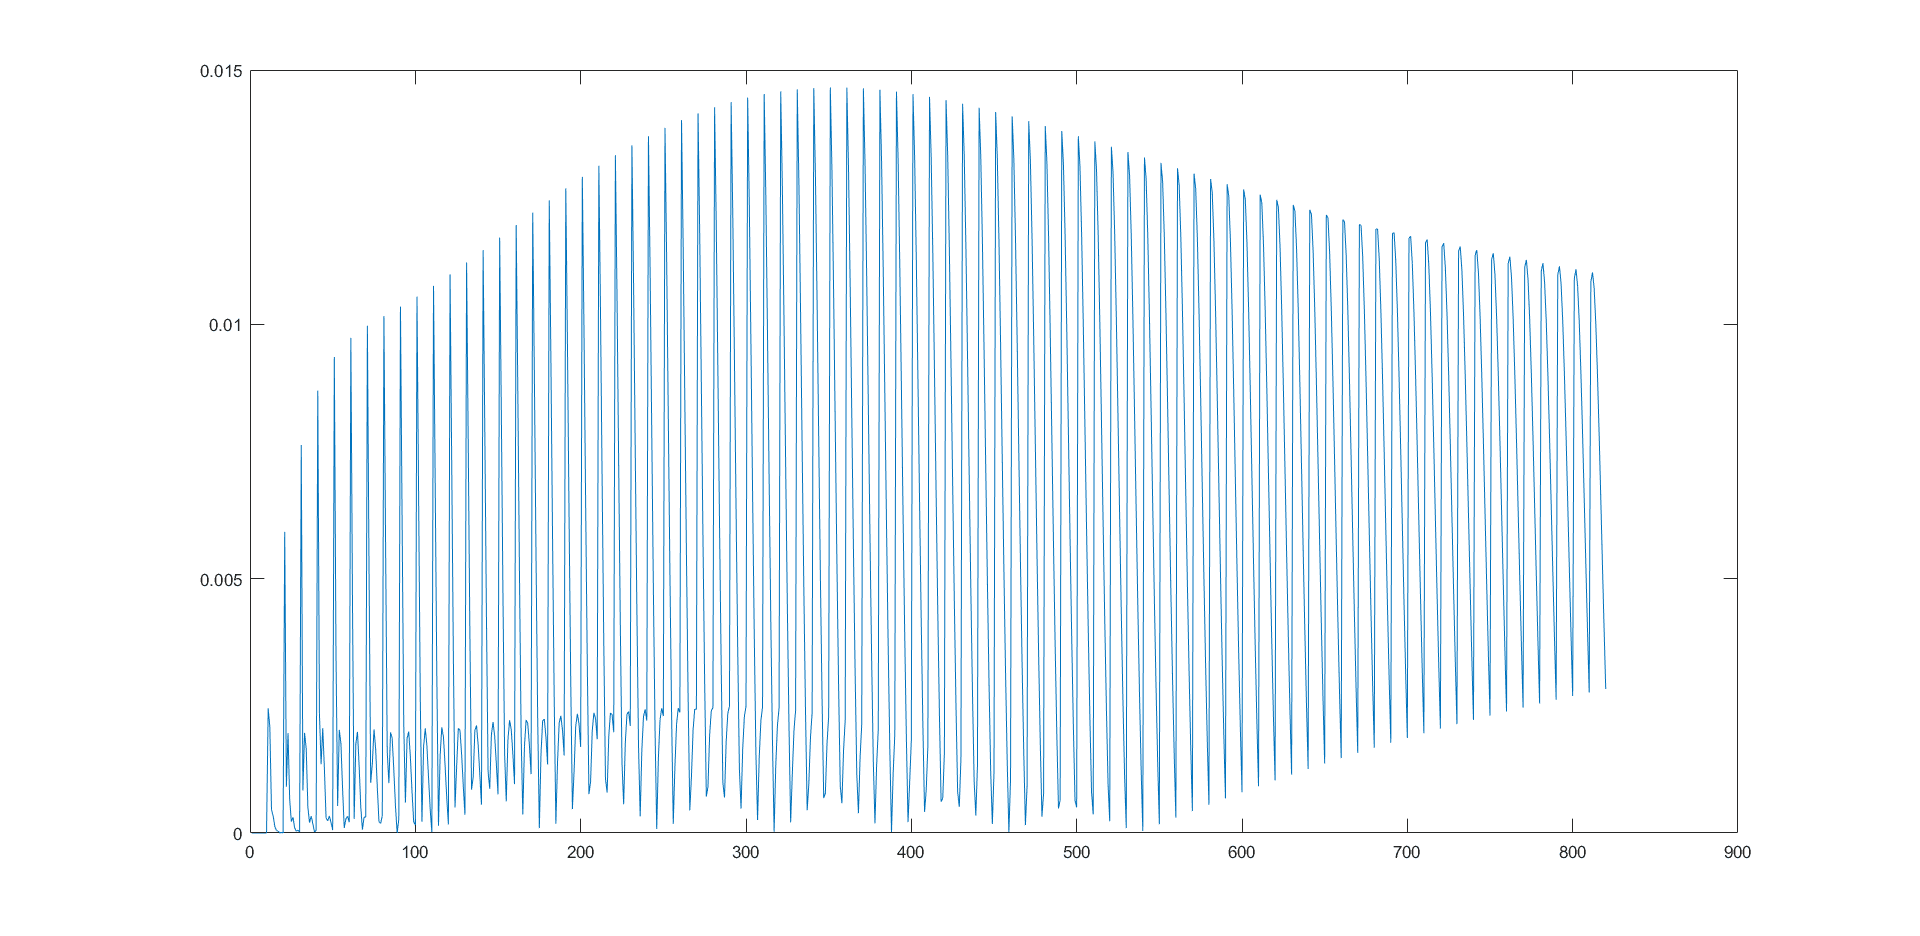
\includegraphics[width=\linewidth]{images/OscillatingMaxDistToRail}
        \label{fig:OMaxDistRail}
        \caption{This plot is similar to \reffig{fig:RandDistToRail} except that the arrangement of the rail in this simulation is in alternating order. The closest distance is again 12mm.}
    \end{figure}
    \begin{figure}[H]
    	\centering
        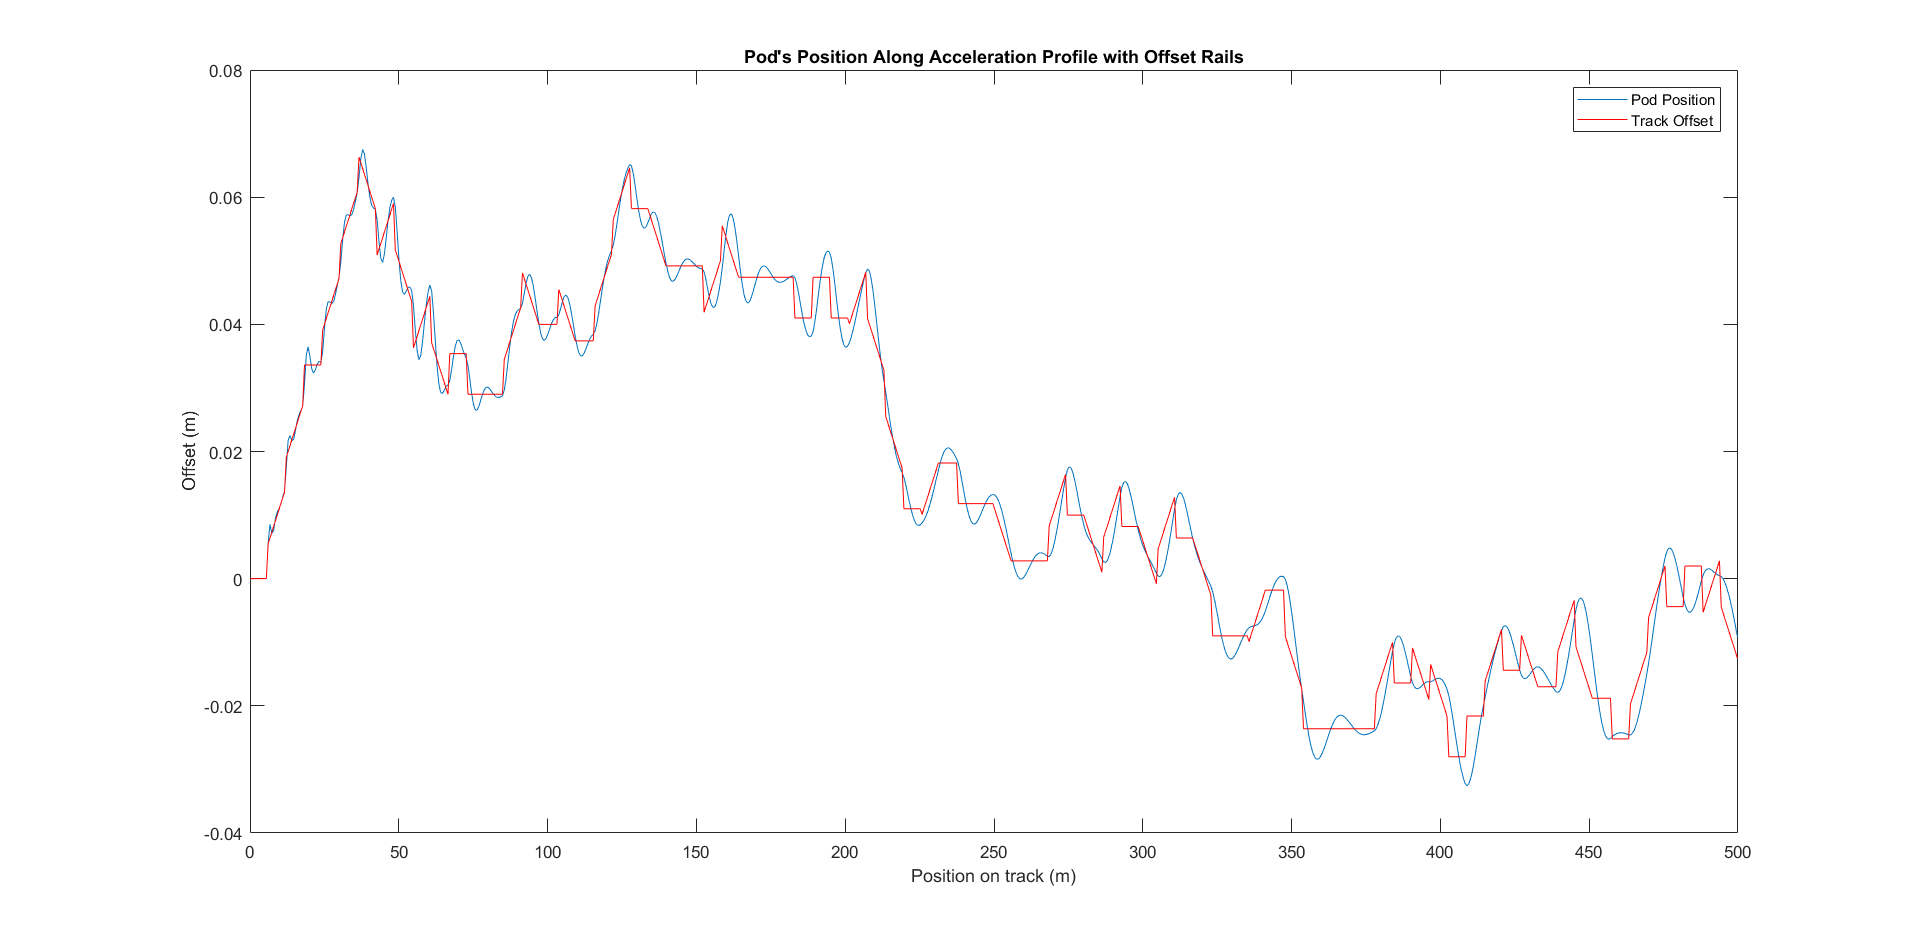
\includegraphics[width=\linewidth]{images/RandPodLateralResponse}
        \label{fig:RandpodLateralResponse}
        \caption{This simulation was done to show how the pod will respond to a rail. In this case the rail offsets were placed in random order.}
    \end{figure}
    \begin{figure}[H]
    	\centering
        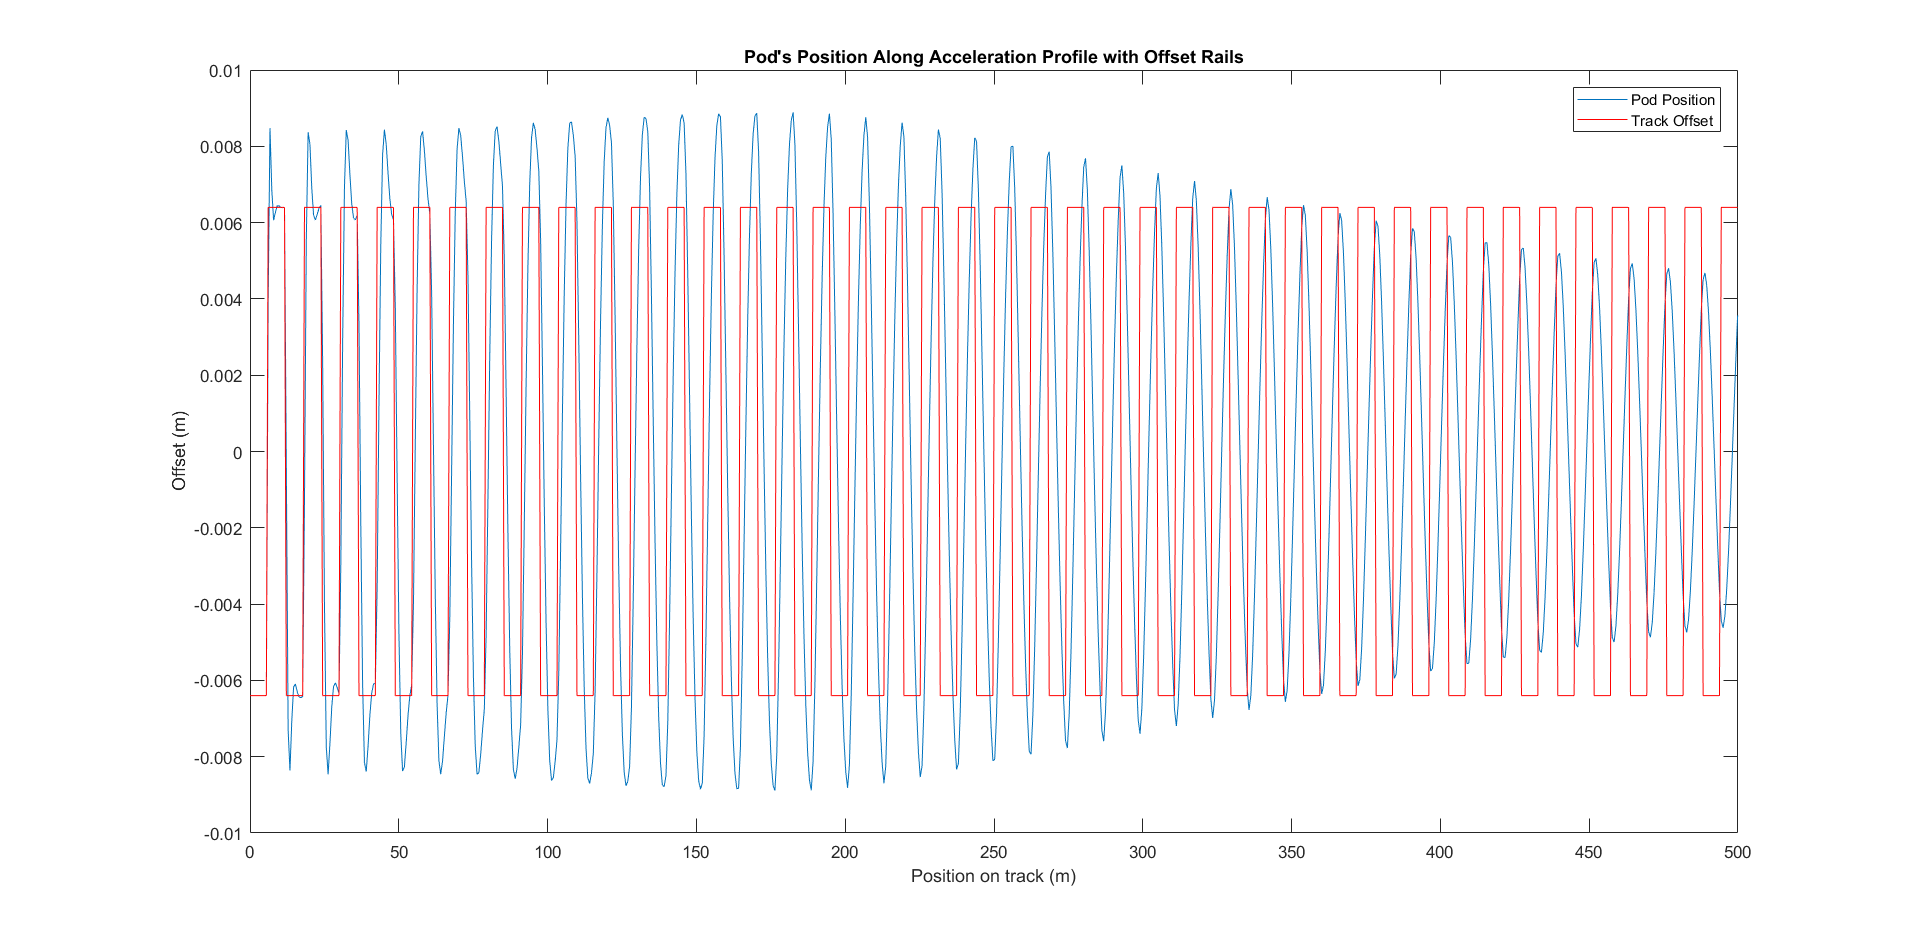
\includegraphics[width=\linewidth]{images/OscillatingPodLateralResponse}
        \label{fig:OPodLateralRespnse}
        \caption{This simulation was done to show how the pod will respond to a rail. In this case the rail offsets were placed in alternating order.}
    \end{figure}
    
    \section{Tests \& Validation }
    \subsection{Damper Coefficient Measurement}
    From our simulations we have determined a damping coefficient which is ideal for our pod. The dampers we have sourced have adjustable damping coefficients, so they must be tested to verify their coefficient is our planned value.\\
    To test these values, we can hang a mass from the damper and observe its behaviour as we let it fall. Using photoelectric distance sensors we can determine the instantaneous velocity of the mass as it falls. Once the mass reaches its steady state velocity, the damper's damping coefficient will be given by:
%     \begin{equation}\label{eq:damper}
	\[
     b = \frac{mg}{v}
    \]
%     \end{equation}
    \subsection{Static Impulse Test}
    The fully-assembled pod will be loaded on an in-house test track and subjected to a lateral impulse. Sensor values and video will then be analyzed to ensure pod is sufficiently damped (i.e., the pod does not oscillate past its equilibrium point more than twice).
    \subsection{Dynamic Integration Test}
    After unit testing is complete, the team plans on doing integration testing on the longest possible track within our capabilities. This track will be used to allow the pod to test its subsystems at speed.\\
    Lateral control will be tested by observing the pod's position when moving along a rail for which there is a deliberately placed offset at the joining of beams.
\end{document}
